\documentclass[a4paper, 12pt]{article}

\usepackage[T2A]{fontenc}
\usepackage[english, russian]{babel}
\usepackage[top=2cm,bottom=3cm,left=1.5cm,right=1.5cm]{geometry}

% Пакет для расширения возможностей
% работы с формулами
\usepackage{amsmath}

% Number equations by section (e.g., 1.1, 1.2)
\numberwithin{equation}{section} 

% Расширение набора
% математических символов
\usepackage{amsfonts}
\usepackage{amssymb}

% Подключим пакет, отвечающий
% за изображения
\usepackage{graphicx}

\usepackage{indentfirst}

\graphicspath{ { ./images/ } }

% Попробуем подвигать текст вручную
% (тут мы будем двигать на титульном листе,
% но аналогичные операции будут работать
% везде в теле документа)
\begin{document}

\title{Отчёт о выполнении лабораторных работ 1.3.1 и 1.3.2 \\
Определение модуля Юнга на основе исследования деформации растяжения. \\
Определение модуля кручения.}
\author{Новиков Александр, Б03-603}
\maketitle

\section{Аннотация}

В работе экспериментально получается зависимость
между напряжением и деформацией (закон Гука)
для одноосного растяжения, 


\section{Определение модуля Юнга по измерениям растяжения проволоки}
\subsection{Теоретические сведения}
Растяжение проволоки соответствует напряженному состоянию вдоль одной оси,
которое описывается формулой:
\begin{equation}
    \frac{F}{S} = E \frac{\Delta l}{l}
    \label{stretch:general_hook}
\end{equation}
Эту формулу можно переписать также в следующем виде:
\begin{equation}
    F = k\Delta l,
\end{equation}
где $k = ES / l$ -- жесткость проволоки.

Измерения производятся на установке Лермантова (рис. \ref{fig:lermantov}).
Считая, что проволока слаборастяжима, используем приближение малых углов
и получаем формулу для расчёта удлинения по показаниям шкалы установки:
\begin{equation}
	\Delta l = \frac{r}{2h} \Delta n
	\label{stretch:length}
\end{equation}

Нагрузка представляет собой только множество грузов,
можем найти её по формуле:
\begin{equation}
	P = Mg
\end{equation}
где $M$ -- масса площадки О со всеми грузами на ней.

Отсюда формулу (\ref{stretch:general_hook}) можно переписать как
\begin{equation}
	\Delta m = \frac{ESr}{2lhg} \Delta n
\end{equation}

\subsection{Методика измерений}
Для определения модуля Юнга используется прибор Лермантова
(рис. \ref{fig:lermantov}).

\begin{figure}[h]
	\centering
	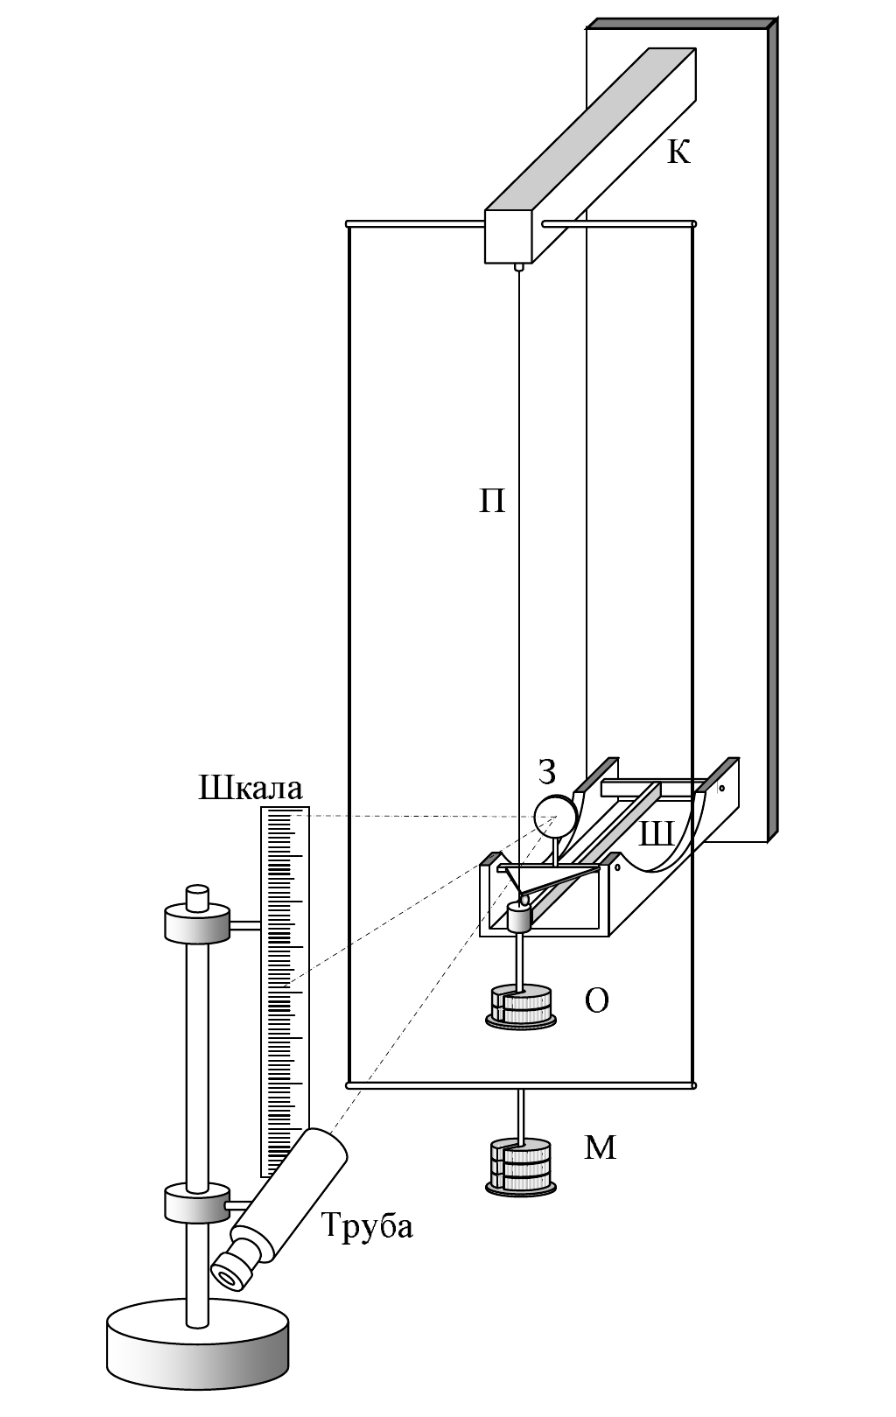
\includegraphics[width=0.5\textwidth]{images/setup1311}
	\caption{Схема прибора Лермантова.}
	\label{fig:lermantov}
\end{figure}

Для исключения деформации кронштейна К на точность измерений
мы меняем натяжение проволоки, перекладывая грузы
с площадки М на площадку О и наоборот - нагрузка остаётся постоянной.

Сведем характеристики установки в таблицу:
\begin{table}[h]
	\centering
	\caption{Параметры прибора Лермантова}
	\begin{tabular}{|c|c|c|c|}
	\hline
	$d_{\text{пр}}$, мм & $r$, мм & $l$, см & $h$, см\\ \hline   % & $\sigma_{\text{пр}}$, Н/мм$^2$
	$0.46 \pm 0.01$            & $15 \pm 1$ & $178 \pm 1$  & $137\pm 2$\\ \hline   % & 900
	\end{tabular}
\end{table}

Оценим максимальную (если повесить все грузы)
и предельную величину нагрузки, приняв,
что разрушающее напряжение равно
$\sigma_\text{пр} = 900 ~ \frac{\text{Н}}{\text{мм}^2}$.
$$P_\text{пр} = (44{,}87 \pm 1{,}95) ~ \text{Н}$$
$$P_\text{max} = (24{,}22 \pm 0{,}03) ~ \text{Н}$$
Согласно полученным значениям, мы можем повесить все грузы.


\subsection{Результаты измерений}


\section{Определение модуля кручения стержня статическим методом}
\subsection{Теоретические сведения}

\subsection{Методика измерений}

\subsection{Результаты измерений}


\section{Определение модуля сдвига при помощи крутильных колебаний}
\subsection{Теоретические сведения}

\subsection{Методика измерений}

\subsection{Результаты измерений}


\section{Заключение}

В работе измерено среднее число частиц, прошедшее через счётчик Гейгера-Мюллера
и проверено выполнение статистических закономерностей, таких как законы
распределения Пуассона и Гаусса, которые наиболее точно описывают распределение
среднего числа частиц, возникшее при обработке данных измерений.

\end{document}